\RequirePackage[2020-02-02]{latexrelease}
\documentclass[times, twoside]{zHenriquesLab-StyleBioRxiv}
%\usepackage{blindtext}
\usepackage{algorithm}
\usepackage{algcompatible}

% Please give the surname of the lead author for the running footer
\leadauthor{Šmelko} 

\begin{document}

\title{MaBoSS for HPC environments: Implementations of the continuous time Boolean model simulator for large CPU clusters and GPU accelerators}
\shorttitle{MaBoSS for HPC environments}

% Use letters for affiliations, numbers to show equal authorship (if applicable) and to indicate the corresponding author
\author[1,\Letter]{Adam Šmelko}
\author[2]{Miroslav Kratochvíl}
\author[3,4,5]{Emmanuel Barillot}
%\author[3,4,5]{Laurence Calzone}
\author[3,4,5,\Letter]{Vincent Noël}

\affil[1]{Department of Distributed and Dependable Systems, Charles University, Prague, Czech Republic}
\affil[2]{Luxembourg Centre for Systems Biomedicine, University of Luxembourg, Esch-sur-Alzette, Luxembourg}
\affil[3]{Institut Curie, Université PSL, F-75005, Paris, France}
\affil[4]{INSERM, U900, F-75005, Paris, France}
\affil[5]{Mines ParisTech, Université PSL, F-75005, Paris, France}
\maketitle

%TC:break Abstract
%the command above serves to have a word count for the abstract
\begin{abstract}
Computational models in systems biology are becoming more important with the advancement of experimental techniques to query the mechanistic details responsible for leading to phenotypes of interest. In particular, Boolean models are well fit to describe the complexity of signaling networks while being simple enough to scale to a very large number of components. With the advance of Boolean model inference techniques, the field is transforming from an artisanal way of building models of moderate size to a more automatized one, leading to very large models. In this context, adapting the simulation software for such increases in complexity is crucial. 
We present two new developments in the continuous time Boolean simulators: MaBoSS.MPI, a parallel implementation of MaBoSS which can exploit the computational power of very large CPU clusters, and MaBoSS.GPU, which can use GPU accelerators to perform these simulations. 
\end {abstract}
%TC:break main
%the command above serves to have a word count for the abstract

\begin{keywords}
Computational Biology | High Performance Computing | Boolean models
\end{keywords}

\begin{corrauthor}
smelko@d3s.mff.cuni.cz, vincent.noel@curie.fr
\end{corrauthor}
\section*{Introduction}
Biological systems are large and complex, and understanding their behavior remains critical to designing new therapies for complex diseases such as cancer. A crucial approach in this endeavor is building computational models from existing knowledge and analyzing them to find intervention points and predict the efficacy of new treatments.
Many different frameworks have been used to describe biological systems, from quantitative systems of differential equations to more qualitative approaches such as Boolean models. While the former seems more adapted to represent complex behavior, such as non-linear dependencies, the latter is being increasingly used because it is capable of representing very large systems.
Many Boolean models have been built to describe biological systems to tackle a variety of problems: from understanding fundamental properties of cell cycle~\cite{faure2006cellcycle,sizek2019boolean} to more advanced properties of cancer~\cite{fumia_carcinogenesis_2013, montagud2022prostate}.

Historically, the task of building Boolean models involved reading an extensive amount of literature and summarizing it in a list of essential components and their interactions. More recently, thanks to advances in databases listing such interactions~\cite{licata2020signor,turei2016omnipath} and to experimental techniques providing information on a bigger number of components, the automatic methods have been designed to infer Boolean formulas from the constraints encoded in the knowledge and the experimental data~\cite{10.1093/bioinformatics/btaa484,chevalier2020synthesis,benevs2023boolean} to build large Boolean models. While this effort faces many challenges, we believe it is the best way to study the large-scale complexity of biological systems. However, in order to analyze the dynamic properties of such large Boolean models, we need to develop efficient simulation tools. In this effort, adapting existing software to modern HPC computing architectures is an important goal. 

Our work focuses on extending MaBoSS~\cite{stoll2012continuous, stoll2017maboss} --- a stochastic Boolean simulator that performs estimations of state probability trajectories based on Markov chains. 
The main contributions of this paper are twofold:
\begin{itemize}
    \item MaBoSS.GPU, a GPU-accelerated implementation of MaBoSS, which is designed to exploit the computational power of massively parallel GPU hardware.
    \item MaBoSS.MPI, a parallel implementation of MaBoSS which can scale to multinode environments, such as large CPU clusters.
\end{itemize}

The source codes of the proposed implementations are publicly available at their respective GitHub repositories\footnote{\url{https://github.com/sysbio-curie/MaBoSS.GPU}} \footnote{\url{https://github.com/sysbio-curie/MaBoSS-env-2.0}}. We also provide the scripts, presented graphs, data and instructions to reproduce the benchmarks in the replication package\footnote{\url{https://github.com/asmelko/gigascience24-artifact}}.

The paper is organized as follows. In the next section, we discuss the MaBoSS algorithm and its complexity. In the following section, we detail the implementation of MaBoSS.GPU and MaBoSS.MPI. In the results section, we present the performance benchmarks of the new implementations. Finally, we conclude the paper and discuss the future work. [TODO - add section refs]


\section*{Background}

We begin with describing the most important aspects of MaBoSS algorithm in order to understand the optimizations described in the next section.  

MaBoSS algorithm takes the Boolean approach for modeling networks which is defined by a Boolean model. A model consists of $n$ nodes which can be in one of two Boolean values: active ($1$) or inactive ($0$). The \emph{state} of the whole modeled system is represented by a vector $S$ of $n$ Boolean values where $S_i$ represents the value of the $i$-th node. We denote the set of all possible states as $\mathcal{S} = \{0, 1\}^n$ and it holds that $|\mathcal{S}| = 2^n$. 

The model interactions are described as transitions between two states. A single state can have multiple transitions to other states; to encode the notion of prioritizing a specific state transition over others, the transitions are assigned a non-negative real value. Simply, a Boolean network generalizes to a directed weighted graph $G = (\mathcal{S}, \rho)$, where $\rho: \mathcal{S} \times \mathcal{S} \rightarrow [0, \infty)$ is a transition function generating \emph{transition rates}. For convenience, it holds that:
\begin{equation}
    \rho(S, S') = 0 \iff \text{there is no transition from}\ S\ \text{to}\ S'
\end{equation}

MaBoSS simulates \emph{asynchronous update strategy}, further restricting the transitions between states. In this strategy, only a single node can change its value in a single transition; i.e., for a transition from $S$ to $S'$, there exists a single node $i$ such that $S_i \neq S'_i$ and for all $j \neq i$, $S_j = S'_j$. Consequently, a state $S$ can have at most $n$ possible transitions.

For each node, a \emph{Boolean logic} $\mathcal{B}: \mathcal{S} \rightarrow [0, \infty)$ is specified. The logic of $i$-th node determines if a state $S$ is allowed to transition to such state $S'$, where only $S_i$ and $S'_i$ differ. If $\mathcal{B}_i(S) = 0$, then the transition is not allowed. Otherwise, the transition is allowed, and the result value determines the transition rate.

This formalization can also be understood as a formal definition of the Continuous-time Markov process. MaBoSS algorithm simulates this process by producing stochastic \emph{trajectories}. A trajectory is a sequence of states $S^0, S^1, \dots, S^k$ and time points $t^0 < t^1 < \dots < t^k$ where $t^0 = 0$ and $S^0$ is the initial state and for each $i \in \{0, \dots, k-1\}$, $S^i$ transitions to $S^{i+1}$ at time $t^{i+1}$. The simulation ends when a state with no outgoing transitions or a maximum simulation time is reached.

Given a state $S$ and time $t$, the pseudocode for a single iteration of a trajectory simulation is as follows:
\begin{algorithmic}[1]
\State Compute transition rates $\rho_1 = \mathcal{B}_1(S), \dots, \rho_n = \mathcal{B}_n(S)$
\State Sample a random number $r$ from $[0, \sum_{i=1}^n \rho_i)$
\State Find $i$ such that $\sum_{j=1}^{i-1} \rho_j \leq r < \sum_{j=1}^{i} \rho_j$
\State Compute $S'$ from $S$ by flipping the $i$-th bit
\State Sample a random number $u$ from $[0, 1]$
\State Compute $\delta t = -(\ln u) / \sum_{i=1}^n \rho_i$
\State Set $S = S'$ and $t = t + \delta t$
\end{algorithmic}

Multiple trajectories are generated to get a good representation of the Markov process. Then, the statistics of the trajectories are computed. These are:

\begin{enumerate}
    \item \emph{Network state probabilities on a time window} --- Trajectory states are divided by their transition times into time windows based on the time intervals specified by a window size $\Delta t$. For each window, the probability of each state is computed as the duration spent in the state divided by the window size. The probabilities of the corresponding windows are then averaged across all subtrajectories.
    \item \emph{Final states} --- The final state of a trajectory is the last state of the trajectory. The sampled states from the trajectories are used to compute the final state distribution.
    \item \emph{Fixed states} --- A state is fixed if it has no outgoing transitions. The sampled states from the trajectories are used to compute the fixed state distribution.
\end{enumerate}

Notably, nodes can be marked as \emph{internal}. The internal nodes are not considered in the statistics computation of time window probabilities and final states. More specifically, before a trajectory is used for statistics computation, the internal nodes are removed from each state in the trajectory.
This feature is helpful for the models where some nodes are used only for simulation purposes and/or are irrelevant to the final results.


\section*{Complexity evaluation and parallelization opportunities of MaBoSS}

MaBoSS algorithm is, in many aspects, very suitable for highly parallel processing. The simulation across multiple trajectories is embarrassingly parallel because the trajectories are independent of each other. Although the statistics computation is slightly more complicated because the intermediate results from separate trajectories need to be reduced to compute the final statistics, the topic of parallel reduction is a well-researched problem with many efficient solutions. 

In this section, we detail the time complexity of the algorithm steps and discuss the parallelization opportunities.

\subsection*{Simulation complexity and parallelization}

Let us start by analyzing the time complexity of one iteration step of the simulation. Suppose a model with $n$ nodes. If we assume that one Boolean logic formula can be evaluated in $\mathcal{O}(n)$, then the computation of transition rates can be done in $\mathcal{O}(n^2)$. The selection of the flipping bit is $\mathcal{O}(n)$ and the rest of the iteration is $\mathcal{O}(1)$. Therefore, the total time complexity of one iteration is $\mathcal{O}(n^2)$. If we simulate $c$ trajectories with an upper bound of trajectory length $u$, the total simulation time is $\mathcal{O}(c \cdot u \cdot n^2)$. 

Using an idealized parallel execution machine (PRAM model with infinite parallelism), we can optimize the algorithm in the following ways: 
\begin{itemize}
    \item All trajectory simulations can be performed in parallel, reducing the time complexity to $\mathcal{O}(m \cdot n^2)$.
    \item A single trajectory iteration can be parallelized. With $n$ processors, the computation of transition rates is achievable in $\mathcal{O}(n)$ time, where each processor would evaluate one Boolean logic formula, and the selection of the flipping bit can be done in $\mathcal{O}(\log{n})$ time using parallel prefix sum. This sums up to $\mathcal{O}(n)$ time for a single iteration. 
\end{itemize}

Overall, using a perfect parallel machine with $c \cdot n$ processors, the simulation time can be reduced to $\mathcal{O}(u \cdot n)$. There is a clear dependency between the trajectory iterations, so $\mathcal{O}(u)$ steps must be performed serially. Realistically, parallelizing an iteration step may prove beneficial only for rather large models when the scheduling overhead and communications cost are lower than the achieved parallelism.

Also, since the trajectory iteration is the main `hot loop' of the whole algorithm (it is executed $c \cdot u$ times), optimizing it as much as possible is imperative. The penalty for the processor handling a cache miss inside each loop can result in the orders-of-magnitude slowdown. This puts a big pressure on the choice of the data representation for the state $S$ and Boolean logic formulas. We discuss this topic in the Implementation section. 

\subsection*{Statistics computation complexity and parallelization}

For the sake of brevity, let us discuss only the time window probabilities computation. The final and fixed states computation performs the same operation but less often because the final and fixed states are computed only from the last state of each trajectory.

The first part of the computation is updating a data structure that holds the durations of states visited in a trajectory. With the choice of a hash map as the data structure, the update can be done in $\mathcal{O}(1)$ time. In the second part, after all trajectories are simulated, the intermediate data structures from the trajectories must be merged into a final one. This can be done in $\mathcal{O}(\log{c} \cdot m)$ time, assuming a serial merging cost of $\mathcal{O}(m)$.

Notably, if the number of states is small enough, or the nodes are dominated by many internal nodes, the hash map can be materialized as a fixed-size array (and be interpreted as a histogram). This would eliminate any memory allocations and the key lookup would be reduced to a simple index function. This optimization is discussed in the next section.

Finally, we use this discussion to detail the specific optimization choices in the implementation of the algorithms.

\section*{Implementation}\label{sec:implementation}

In this section, we describe the high-level overview of MaBoSS.GPU and MaBoSS.MPI implementation.

\subsection*{MaBoSS.GPU}
Porting MaBoSS algorithm to GPUs poses an interesting task from the optimizations perspective. A simple rewrite to an annotation-based tool, such as OpenACC, may not be the most optimal strategy due to the usage of complex data structures, such as hash maps and expression trees, that are not well suited for GPU hardware. We divided the implementation into two parts: the bare \emph{simulation} and the trajectory \emph{statistics computation}. 

\subsubsection*{Simulation}

The simulation part is the most computationally demanding part of the CPU MaBoSS implementation. The preliminary performance reports show that around $30-80\%$ of the MaBoSS runtime (depending on the model) is spent in the evaluation of Boolean formulas. This evaluation is carried out in a recursive call over an expression tree. This approach is not well suited for a CPU cache because the whole tree may span multiple cache lines and, apart from other issues, its traversal may easily result in a major cache miss ratio~\cite{karlsson2000prefetching}. The GPUs are even more susceptible to this problem because they have a lower cache per core ratio. We took this as a starting point for our optimizations.

There are multiple ways to tackle the problem of bad cache performance of the expression tree. One can either use a linked data structure that is more cache-friendly, such as the van Emde Boas tree layout~\cite{van1975preserving}, or perhaps represent the Boolean formulas as a compact continuous array with an ad-hoc layout. In our approach, we take one step further by utilizing the \emph{runtime compilation of GPU code}~\cite{nvrtc}. Using this technique, instead of building the expression tree for the Boolean formulas, we compile the formulas into a native binary code that can be executed directly on the GPU. The main advantage of this approach is that the formulas are encoded in the instructions instead of being stored in the memory. This way, the formulas would not need to be fetched from memory multiple times during the application runtime. The other advantage is that the compiler can optimize the GPU code to utilize the GPU hardware more efficiently. 

The major drawback of the runtime compilation is its speed. The compilation takes magnitudes longer than the building of the expression trees. On the other hand, the formulas compilation is executed only once at the beginning of the simulation and the compiled code is reused for the whole simulation. In theory, the compilation time can get amortized well by the overall simulation and statistics computation time for big enough models.

In our implementation, we decided to assign a single GPU thread to a single trajectory. We mentioned in the previous section, that a work distribution, where multiple threads would work on a single trajectory, may be beneficial for large models. However, this can not be implemented trivially without creating a thread divergence in the transition rates computation (which is usually penalized by a completely serialized execution anyway). This optimization requires a clever rewrite of the Boolean logic, which we leave for future work.

\subsubsection*{Statistics computation}

The CPU implementation of this part of the algorithm heavily relies on the usage of hash maps. They are used to store node states as the keys, and the values may be the state occurrences or their average timespan in the trajectories, depending on the specific statistics computation. We will focus on the probability distribution of trajectory states since it is the most computationally demanding part of the statistics computation and the optimizations used for this part apply to the other statistics computations as well.

The optimization of this step relies on the fact that the typical number of non-internal nodes in a real-world MaBoSS model rarely exceeds 10 nodes regardless of the total number of nodes. The relatively low number of states generated by non-internal nodes allows us to materialize the whole histogram as a fixed-size array. The states are no longer stored as the keys --- rather, a hash function is used to map the states to the histogram array indices. We use a simple hash function with bit masking and shifting to extract and compact non-internal nodes from the state representation. Further, we use well-known GPU histogram optimizations, such as shared memory privatization and atomic operations, to improve the performance of the histogram computation.

\subsection*{MaBoSS.MPI}
Since MaBoSS.MPI and MaBoSS.GPU projects were developed in parallel, the MPI implementation of MaBoSS is based on the original CPU code. Same as in GPU code, CPU implementation also assigns a single thread to a single trajectory. The MPI implementation simply extends this distribution of work among multiple MPI nodes, adding the second layer of parallelism. 

In summary, MaBoSS.MPI evenly distributes individual trajectories first on MPI nodes and then on the corresponding CPU cores, assuming the MPI nodes are homogenous. Once the trajectories are simulated and the statistics are computed for each MPI node, the intermediate data are reduced into a final result using MPI collective operations.


% MaBoSS' CPU implementation already offered parallelism, allowing to use multiple CPU cores to compute the multiple trajectories. However, this implementation stays limited to a single machine CPU, and its scalability suffers from a very intensive memory usage. Furthermore, with the increasing number of nodes in Boolean models, the need for very large number of trajectories leads to large simulation time. 
% To tackle this, we decided to extend this implementation and add another layer of parallelism using MPI. In this implementation, the simulation of the trajectories is not only distributed on multiple cores, but on the multiple cores of multiple MPI nodes. By using this implementation, we are able to exploit the large CPU clusters available in HPC centers. 
% The implementation of this MPI implementation is straightforward, and consists in distributing the invidivual trajectories even further, first on MPI nodes and then on the CPU cores of the MPI node. Once the trajectories are simulated, the statistics are first computed for each MPI nodes, and then the global results is computer from the results of each MPI nodes. 


\section*{Results}

To evaluate the discussed optimizations, we present the results of performance benchmarks for MaBoSS.GPU and MaBoSS.MPI by comparing their runtimes against the original CPU implementation. To get comprehensive results, we used real-world models and synthetic models with varying sizes.

\subsubsection*{Benchmarking Methodology}

For the benchmarks, we used $3$ real-world models with varying model sizes spanning from $10$ nodes to $133$ (\texttt{cellcycle}~\cite{faure2006cellcycle}, \texttt{sizek}~\cite{sizek2019boolean} and \texttt{Montagud}~\cite{montagud2022prostate}). In order to test the scalability of the GPU and MPI implementation, we also created a synthetic models with up to $1000$ nodes. Synthetic models are designed in a way such that the length of each trajectory is predictable, and the models have no stable states. Also, the number of non-internal nodes is kept low (10 nodes) to enable the usage of the histogram optimization.

The GPU implementation benchmarks were run on a datacenter-grade NVIDIA Tesla A100 GPU and a consumer-grade NVIDIA RTX 3070 Laptop GPU. The CPU implementation benchmarks were run on a 32-core Intel Xeon Gold 6130 CPU with multithreading. The CPU implementation was compiled with GCC 13.2.0, and the GPU implementation was compiled with CUDA 12.2. Each measurement was repeated $10$ times, and the average runtime was used for the final results after removing the outliers.

The MPI implementation benchmarks were run on the MareNostrum 4 supercomputer.


\subsection*{MaBoSS.GPU}

\begin{figure}
    \centering
    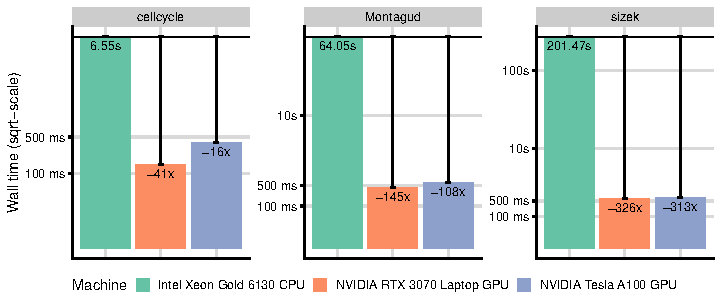
\includegraphics[width=\linewidth]{Figures/real.pdf}
    \caption{Wall time comparison of CPU and GPU implementations on real-world models. Each model is simulated with 1 million trajectories.}
    \label{fig:real}
\end{figure}

In Figure~\ref{fig:real}, we compare the wall time of the CPU and GPU implementations on real-world datasets. The GPU implementation is faster than the CPU implementation on all models, and the speedup shows to be more significant on the models with more nodes and longer trajectories. On Montagud model with 133 nodes but a relatively short average trajectory, we achieve $145\times$ speedup. On a slightly smaller Sizek model with a longer average trajectory, the speedup is up to $326\times$. 

\begin{figure}
    \centering
    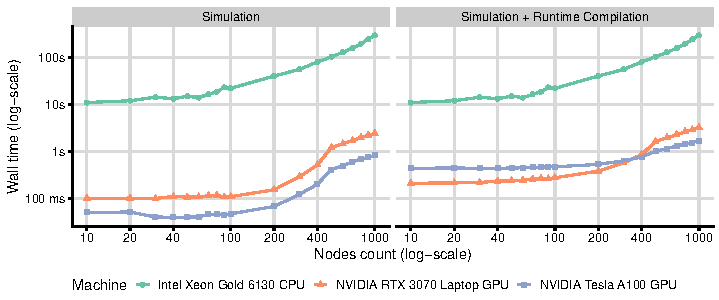
\includegraphics[width=\linewidth]{Figures/nodes.pdf}
    \caption{Wall time comparison of CPU and GPU implementations on synthetic models. Each model is simulated with 1 million trajectories.}
    \label{fig:synth}
\end{figure}

Figure~\ref{fig:synth} shows much finer performance progression on synthetic models. On the left subplot, the runtime compilation is filtered out to show the pure simulation performance. We can see that the CPU variant starts to progress steeper at around the $100$ nodes boundary. We can expect that the implementation hits the cache size limit and fetching the required data from the memory comes with more overhead. The same can be observed in the GPU variant, but at $200$ nodes and with more drastic increase. This observation corresponds to a much more significant performance penalty when fetching data from the GPU memory. Overall, this suggests that the optimization of dividing transition rates computation among multiple threads mentioned in the previous section may provide a significant speedup for bigger models as it alleviates the register pressure.

\begin{figure}
    \centering
    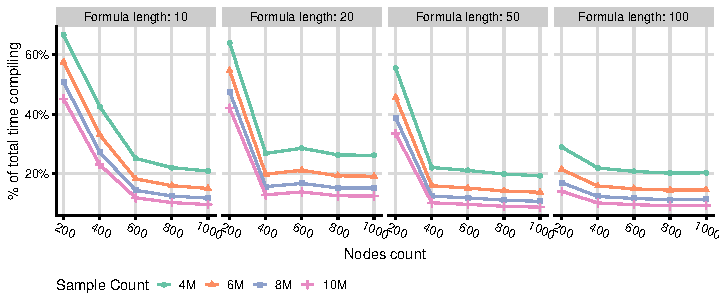
\includegraphics[width=\linewidth]{Figures/nodes-compilation-big-NVIDIA Tesla A100 GPU.pdf}
    \caption{The time spent in the runtime compilation of the Boolean formulas simulating models with varying numbers of nodes, trajectories, and formula lengths.}
    \label{fig:comp}
\end{figure}

The right subplot shows the total runtime of the GPU implementation. Comparing the subplots shows that the runtime compilation ratio decreases with increasing model size. Figure~\ref{fig:comp} offers more detailed benchmarks for this scenario, run on the NVIDIA Tesla A100 GPU. The compilation time is linearly dependent on the number of nodes and formula lengths (measured in the number of occurring nodes). Notably, as soon as the simulation becomes more complex, i.e., by increasing the number of nodes or simulated trajectories, the compilation time becomes less than $10\%$ of the total runtime, even for the models with unrealistically long formulae. This suggests that the runtime compilation is a viable optimization for bigger models.


\subsection*{MaBoSS.MPI}

\begin{figure}%[tbhp]
\centering
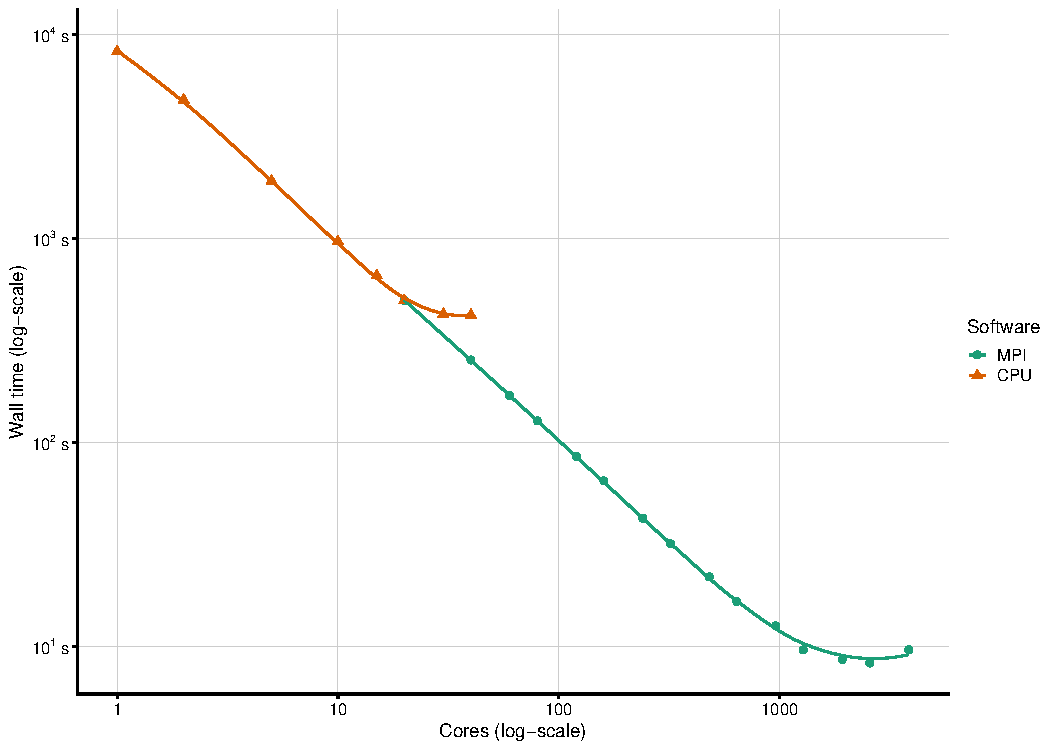
\includegraphics[width=.8\linewidth]{Figures/sizek_mpi.pdf}
\caption{Scalability results of MPI implementation on Sizek model with 20 cores per MPI node.}
\label{fig:sizek_results}
\end{figure}

Figure~\ref{fig:sizek_results} shows the efficiency of the MPI implementation on the Sizek model. We ran multiple suites, ranging from a single MPI node up to 192 nodes, each running 20 cores. We can observe a close-to-linear speedup of up to 64 MPI nodes (1280 cores), and a plateau for larger suites (Figure~\ref{fig:sizek_results}, green). This can be explained by hitting a bottleneck in parallelization overhead and MPI communication cost when the problem is divided into too many small parts.

\begin{figure}%[tbhp]
\centering
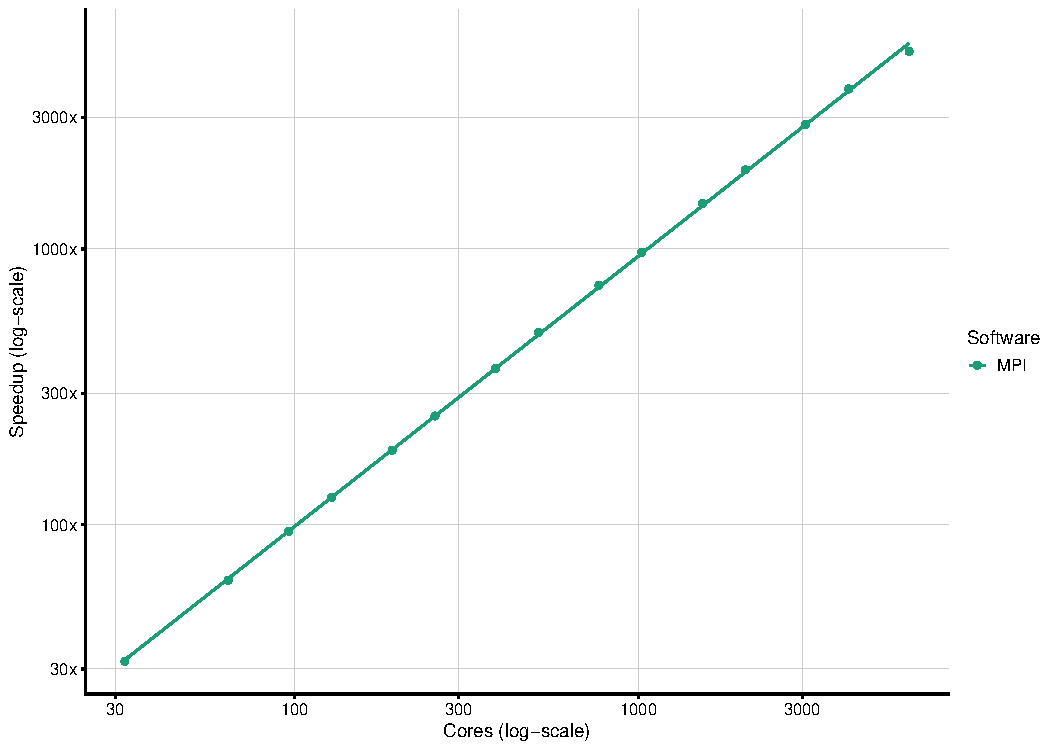
\includegraphics[width=.8\linewidth]{Figures/synth_mpi_speedup.pdf}
\caption{Speedup scaling of MPI implementation on a synthetic model with 1000 nodes and 32 cores per MPI node.}
\label{fig:synthetic_results}
\end{figure}

To stress the scalability of the implementation, we also used a synthetic model with 1000 nodes (see Figure~\ref{fig:synthetic_results}). We simulated this model on 32 cores per MPI node, on 1 to 192 nodes (32 to 6144 cores). With this configuration, the simulation time decreases from 20 hours on 1 MPI node to 430 seconds on 192 nodes. As we hypothesized, a decline in the speedup was not observed in larger simulations. 

% We simulated a cell cycle model by Sizek et al.\cite{sizek2019boolean} (Figure~\ref{fig:sizek_results}). A comparison of execution times of MaBoSS v2.5.3 and v2.4.0 using 40 cores and one million individual simulations showed a considerable (3×) speed-up between the pre- and post-optimisation versions, which is mostly due to optimised memory usage (figure 2, purple vs red). We used the same test with the MPI implementation of MaBoSS, using 20 cores for each MPI node, from 1 MPI node up to 192 MPI nodes. We can observe a very good speedup (>50x) up to 64 MPI nodes (1.28k cores), and a plateau for larger setups (Figure 7, green). This is probably due the very short simulation time (10s) for that setup and the minimum overhead for such a parallel simulation, and needs testing on larger simulations.


% In order to explore larger model sizes, we created a synthetic model with 1000 nodes (Figure~\ref{fig:synthetic_results}). We simulated this model on 32 cores per MPI node, on 1 to 192 MPI nodes (32 to 6144 cores). With this dataset, the simulation time goes from 20 hours on 1 MPI node to 430 seconds on 192 nodes. As we hypothesised, with larger simulation times, a decline in the speedup was not observed as in the previous example 
% The MaBoSS benchmarking measurements described in this section were performed on MareNostrum 4.

% \begin{figure}%[tbhp]
% \centering
% 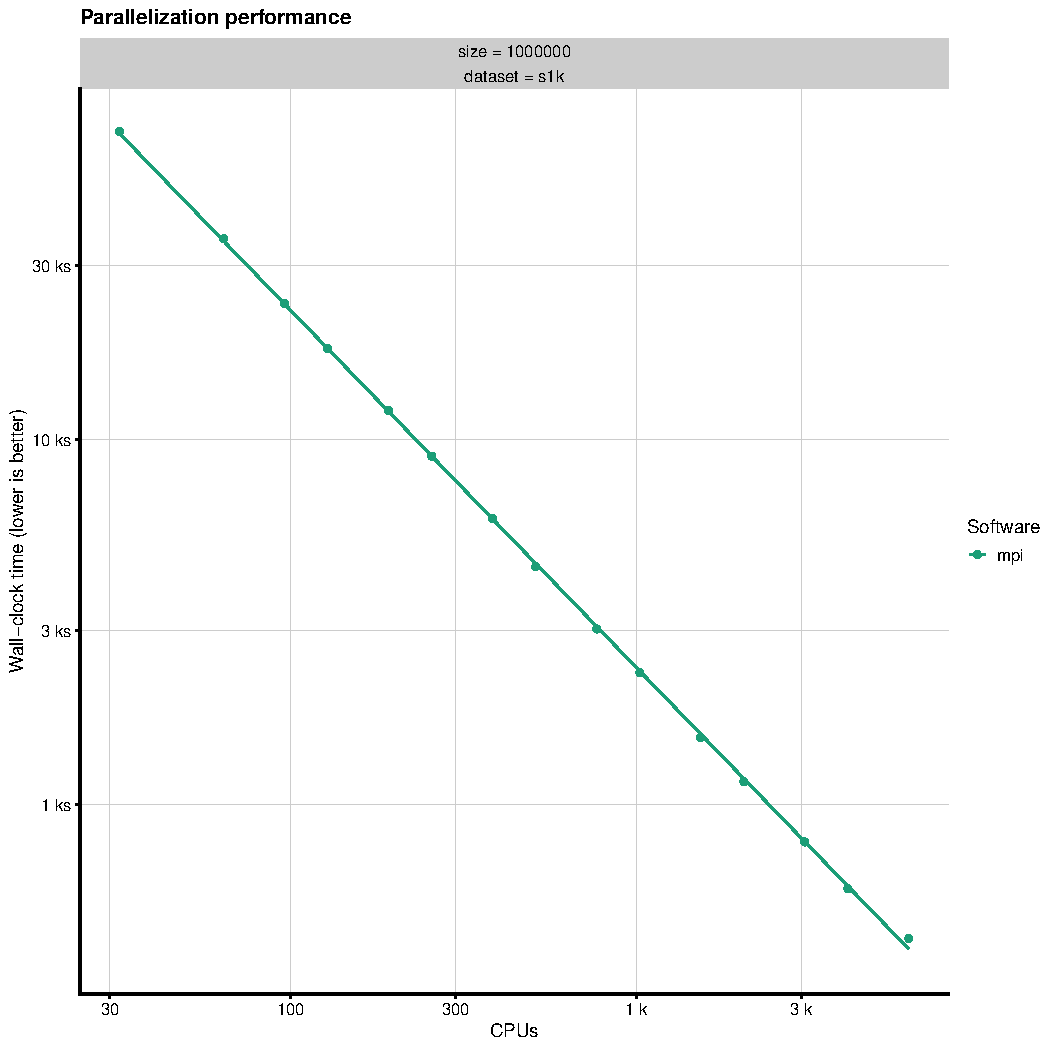
\includegraphics[width=.8\linewidth]{Figures/large_model.pdf}
% \caption{Scalability results for synthetic model with 1000 nodes}
% \label{fig:synthetic_results}
% \end{figure}

%\begin{figure}%[tbhp]
%\centering
%\includegraphics[width=.8\linewidth]{Figures/Figure_1}
%\caption{Placeholder image of Iris with a long example caption to show justification setting.}
%\label{fig:computerNo}
%\end{figure}

\section*{Conclusions}

In this work, we presented two new implementations of MaBoSS tool, a continuous time Boolean model simulator, designed for HPC environments:  MaBoSS.GPU which is designed to exploit the computational power of massively parallel GPU hardware, and MaBoSS.MPI which enables MaBoSS to scale to many nodes of HPC clusters. We evaluated the performance of these implementations on real-world and synthetic models and demonstrated that both variants are capable of providing significant speedups over the original CPU code. The GPU implementation shows $145-326\times$ speedup on real-world models, and the MPI implementation delivers a close-to-linear strong scaling on big models.

Overall, we believe the new MaBoSS extensions will enable the simulation of large, automatically generated models and will be a valuable tool for the systems biology community.

\subsection*{Future work} 

As mentioned in the discussion section, the next steps in the development of MaBoSS.GPU would be to parallelize the iteration step of the simulation. This requires a different representation of Boolean formulas, which would not pose any thread divergence, probably by substituting runtime compilation with an in-memory data structure. This optimization could potentially decrease the register pressure created by holding the state data and thus increase the performance of huge models with hundreds of nodes.

Furthermore, many parallelization methods used in GPU implementation could be backported to the CPU implementation, increasing the overall usability of MaBoSS running on systems without GPU accelerators. 

Finally, to enable the simulation of extra-large models with thousands of nodes at billions of samples, the two presented parallelization methods could be combined into a single high-performance solution by running GPU implementation on multiple MPI nodes.


\begin{acknowledgements}
We thank Laurence Calzone and Gautier Stoll for their guidance and fruitful discussions.
\end{acknowledgements}

\begin{funding}
This work was supported by the European Commission under the PerMedCoE project [H2020-ICT-951773] and SVV project number 260 698.
\end{funding}


\section*{Bibliography}
\bibliography{bibliography}

%% You can use these special %TC: tags to ignore certain parts of the text.
%TC:ignore
%the command above ignores this section for word count
\onecolumn
\newpage

%%%%%%%%%%%%%%%%%%%%%%%%%%%%%
% Supplementary Information %
%%%%%%%%%%%%%%%%%%%%%%%%%%%%%
%\captionsetup*{format=largeformat}
%\section{Something about something} \label{note:Note1} 
%Something

%TC:endignore
%the command above ignores this section for word count

\end{document}
